\section{Conception}

Ce chapitre contient la conception de l'intégration des nombres complexes dans COJAC \cite{COJAC}.

\subsection{Approche}
\label{sec:complex_approach}

Comme expliqué dans la section \ref{sec:cojac_integration}, l'intégration des nombres complexes peut se faire à l'aide de deux mécanismes différents:
\begin{itemize}
    \item Behaviour: réinterprétation des \textit{floats} et des \textit{doubles}.
    \item Wrapper: remplacement des \textit{floats} et des \textit{doubles} par un wrapper.
\end{itemize}

L'intégration des nombres complexes se fera en utilisant un wrapper afin de pouvoir garder la \textit{double precision}.

\subsection{Comparaison}
\label{sec:complex_design_comparison}

La comparaison entre les nombres complexes est un problème important. Toutes les comparaisons entre les nombres sont faites à l'aide d'une même opération et il faut aussi que les comparaisons entre des nombres purement réels soient respectés. Ainsi si on compare des nombres complexes (avec une partie imaginaire), il n'y a pas forcément de valeurs de retour adaptées car il n'y a pas d'ordre total avec les nombres complexes. Cette situation peut être montrée avec l'exemple de code suivant:

\begin{minted}{Java}
double a = ...;
if (a == 0) {
    System.out.println("a = 0");
} else {
    System.out.println("a != 0");
}
\end{minted}

Si la variable \textit{a} est purement réelle, ce code doit fonctionner. Cependant il y a un problème si la variable \textit{a} est complexe. Pour cet exemple, la valeur de \textit{a} sera \textit{2i}. Lorsque le remplacement de cette opération est faite, la méthode doit comparer ces deux nombres (\textit{2i} et 0) et retourner une valeur parmi les trois suivantes:

\begin{itemize}
    \item \textit{2i} < 0
    \item \textit{2i} = 0
    \item \textit{2i} > 0
\end{itemize}

Cependant, aucune de ces réponses n'est vraie. Il est possible de créer une méthode magique pour gérer les égalités, mais ceci nécessitera que l'application cible soit modifiée pour réaliser la comparaison.

Comme aucun des deux choix n'est complètement satisfaisant, une option supplémentaire pour COJAC \cite{COJAC} sera disponible pour choisir le comportement des comparaisons. Ces deux modes différents sont détaillés dans la section \ref{sec:complex_design_modes} suivante.

\subsection{ToString and fromString}

Il a été décidé que le \textit{toString} écrirait le nombre sous sa forme complexe. Ceci peut provoquer une erreur si l'application cible utilise un format strict. Il est surtout important que le \textit{toString} du wrapper puisse être converti en wrapper à nouveau. Ainsi les méthodes \textit{Float.parseFloat} et \textit{Double.parseDouble} doivent aussi fonctionner avec le résultat du \textit{toString} du wrapper.

\subsection{Modes}
\label{sec:complex_design_modes}

Il n'y a pas de comportement idéal pour implémenter la comparaison (cf section \ref{sec:complex_design_comparison}) et le cast en double. Ainsi, les deux modes différents sont détaillés dans cette section. Une synthèse et des exemples comparent les résultats de ces différentes approches.

\subsubsection{Mode normal}

Dans le mode normal, la comparaison se fera d'abord avec la partie réelle, puis avec la partie complexe. Ainsi \textit{2 - i} sera considéré comme plus petit que \textit{2}. Le cast d'un nombre complexe en double provoquera la perte de la partie imaginaire.

Ce mode a l'avantage suivant:
\begin{itemize}
    \item L'application cible n'a pas ou peu besoin de modifications pour fonctionner. Ceci respecte au maximum l'ordre établi entre les nombres réels.
    \item Les méthodes magiques créées pour le mode strict sont aussi disponibles en mode normal. Ces méthodes sont expliquées dans la section \ref{sec:complex_design_modes_strict}.
\end{itemize}

Il possède également les inconvénients suivants:
\begin{itemize}
    \item Un ordre total est défini alors qu'il n'existe pas mathématiquement. Ceci peut conduire à des comparaisons donnant un résultat mathématiquement faux et produire des incohérences.
    \item La partie imaginaire peut être perdue sans le remarquer car cela ne provoquera aucune erreur.
\end{itemize}

\subsubsection{Mode strict}
\label{sec:complex_design_modes_strict}

Quant à lui, le mode strict offrira une comparaison mathématiquement correcte. La comparaison entre deux nombres purement réels donnera toujours un résultat. La comparaison entre deux nombres complexes égaux donnera également un résultat correct. Dans les autres cas, une exception sera générée.

Lors du cast d'un nombre complexe en nombre réel, la présence d'une partie imaginaire générera une erreur. S'il n'y a qu'une partie réelle, le cast fonctionnera.

De plus, une méthode magique permettra de vérifier l'égalité de deux nombres complexes. Elle retournera un booléen même en cas d'inégalité. Deux méthodes magiques permettant de garder seulement la partie réelle ou imaginaire d'un nombre complexe sera aussi disponible et permettra à l'utilisateur d'implémenter lui-même la comparaison entre les nombres complexes.

Ce mode offre les avantages suivants:
\begin{itemize}
    \item La comparaison est mathématiquement correcte. Ainsi, l'utilisateur est conscient des problèmes qui peuvent se produire lorsqu'il travaille avec les nombres complexes.
    \item L'usage des méthodes magiques permet une plus grande flexibilité avec les nombres magiques.
\end{itemize}

Ce mode a aussi l'inconvénient suivant:
\begin{itemize}
    \item L'application cible doit être écrite en tenant compte des fonctions magiques de COJAC \cite{COJAC}.
\end{itemize}

\subsubsection{Exemples}

Voici plusieurs exemples montrant la différence entre le mode normal et le mode strict.

Le premier exemple trie un tableau de nombres complexes, puis calcule leur valeur absolue. Le résultat obtenu est:
\begin{itemize}
    \item Mode normal: le code s'exécute et le tableau final n'est plus trié.
    \item Mode strict: une erreur est générée lors de l'appel à la méthode \textit{Arrays.sort}, parce qu'une comparaison est effectuée avec des nombres complexes contenant une partie imaginaire.
\end{itemize}

\begin{minted}{Java}
double[] sorted_positives = ... // ex: new double[]{2 + 3i, 3, 1};
Arrays.sort(sorted_positives); // sorted_positives = [1, 2 + 3i, 3]
double[] sorted_abs = new double[sorted_positives.length];
for (int i = 0; i < sorted_positives.length; i++){
    sorted_abs[i] = Math.abs(sorted_positives[i]);
}
// sorted_abs = [1, 3.6, 3]
\end{minted}

Le second exemple cast un double en int. Le résultat est le suivant:
\begin{itemize}
    \item Mode normal: a est égal à la partie imaginaire du nombre (a = 2);
    \item Mode strict: une exception est générée à cause de la perte de la partie imaginaire
\end{itemize}

\begin{minted}{Java}
double d = Math.sqrt(-1) + 2; // 2 + i
int a = (int) d;
\end{minted}

Avec une méthode magique, le même résultat peut aussi être obtenu avec le mode strict:
\begin{itemize}
    \item Mode normal ou strict: a est égal à la partie imaginaire du nombre (a = 2);
\end{itemize}

\begin{minted}{Java}
double d = Math.sqrt(-1) + 2; // 2 + i
int a = (int) COJAC_MAGIC_getReal(d);
\end{minted}

\subsubsection{Synthèse}

Le mode normal nécessite aucune modification pour démarrer le programme. Cependant, il peut y avoir des erreurs de logique. Le mode strict garanti un comportement mathématiquement correct et limite le nombre d'erreurs. Cependant, il est nécessaire d'utiliser des méthodes magiques et, par conséquent, de modifier le code de l'application cible. Les méthodes magiques sont aussi disponibles en mode normal et il est ainsi possible de faire la transition du mode normal au mode strict par étapes. Ces méthodes magiques peuvent aussi être utilisés pour avoir un comportement plus sûr à un endroit spécifique du code.

\subsection{Librairie disponible}

La librairie \textit{commons-math3} est déjà disponible en Java pour gérer les nombres complexes \cite{apache-complex-documentation}. Elle possède beaucoup de fonctionnalités et implémente déjà la grande majorité des opérations mathématiques nécessaires. De plus, cette librairie fait déjà partie des dépendances de ce projet. Elle sera ainsi utilisée pour implémenter les nombres complexes.

\subsection{Diagramme de classes}

Toutes les méthodes abstraites du \textit{ACojacWrapper} seront implémentées en plus de plusieurs autres méthodes. De plus, une nouvelle méthode sera ajoutée au \textit{ACojacWrapper} afin de pouvoir supporter la méthode \textit{Math.cbrt}. Les méthodes du wrapper sont surchargées pour retourner un \textit{WrapperComplexNumber} à chaque fois pour simplifier les tests. Toutes les méthodes de la classe \textit{WrapperComplexNumber} qui sont visibles sur le diagramme de classes ont été implémentées.

\begin{minipage}{\linewidth}
\makebox[\linewidth]{
    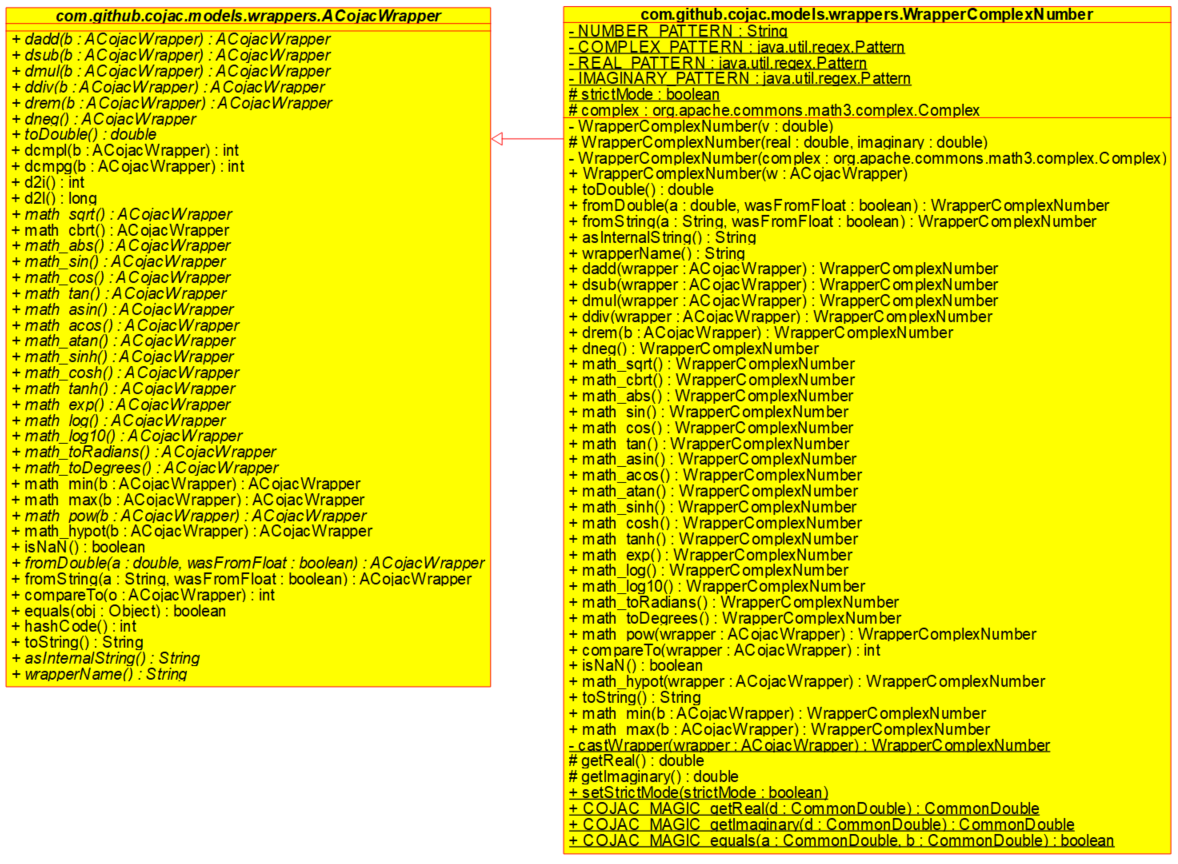
\includegraphics[width=\linewidth]{complex_numbers/class_diagram.png}
}
\captionof{figure}{Diagramme de classes de l'intégration des nombres complexes}
\label{fig:class_diagram}
\end{minipage}